% Title: Report LaTex File: Software Development
% Auther: DC Eksteen
% Student Number: 22623906
% Contact: 22623906@sun.ac.za
% Date: 2022/09/14
% Version: 2.0

\chapter{Software Development}
\label{ch:software}

\vspace*{-0.5cm}

The software that was developed for this project was written in object orientated Python 3. The software is aimed at Linux operating systems, as it leveraged the Bluez stack for \ac{ble} communication. The software was then deployed on a Raspberry Pi 3 B+ single-board computer in order to utilise the \ac{gpio} pins. Ergasia was chosen as the name for the trainer model.

\vspace*{-0.5cm}

\section{Structure}

A Raspberry Pi was selected as the micro-controller base for the trainer. This means that the application will run on Raspberry Pi OS (previously called Raspbian), which is a 32-bit Unix-like operating system based on the Debian Linux distribution that was specifically developed for the Raspberry Pi. Subsequently, the application software was developed to work with standard Linux system architecture to achieve the required functionality.

Within the Linux system, the \ac{dbus} was used as a message based middleware mechanism delivering \ac{ipc} calls between processes running within the active session. The \ac{dbus} is accessed with Python using the GLib library.

The main code section was written to rely on interrupts and timers rather than polling. This means that the \ac{cpu} is only utilised when an event occurs, making the application less resource intensive and faster to respond to rapid events.

\section{\acl{ble} Communication}

Following an object-orientated approach, the following classes were defined for the different elements required by the \ac{ble} \ac{gatt} specifications:

\begin{itemize}
	\item Service
	\vspace*{-0.3cm}
	\item Characteristic
		\vspace*{-0.3cm}
	\item Descriptor
		\vspace*{-0.3cm}
	\item Advertisement
\end{itemize}

When the application initialises, multiple objects of these classes are created with the various information that is required for the \ac{ftms} and \ac{dis} \ac{ble} services. The Raspberry Pi then advertises itself as a peripheral with access to these services. This advertisement can then be read and responded to by nearby master devices. Figure~\ref{fig:blt} shows the advertisement read by Light Blue, a \ac{ble} master emulating application.

\begin{figure}[H]
	\centering
	\begin{subfigure}{.4\textwidth}
		\centering
		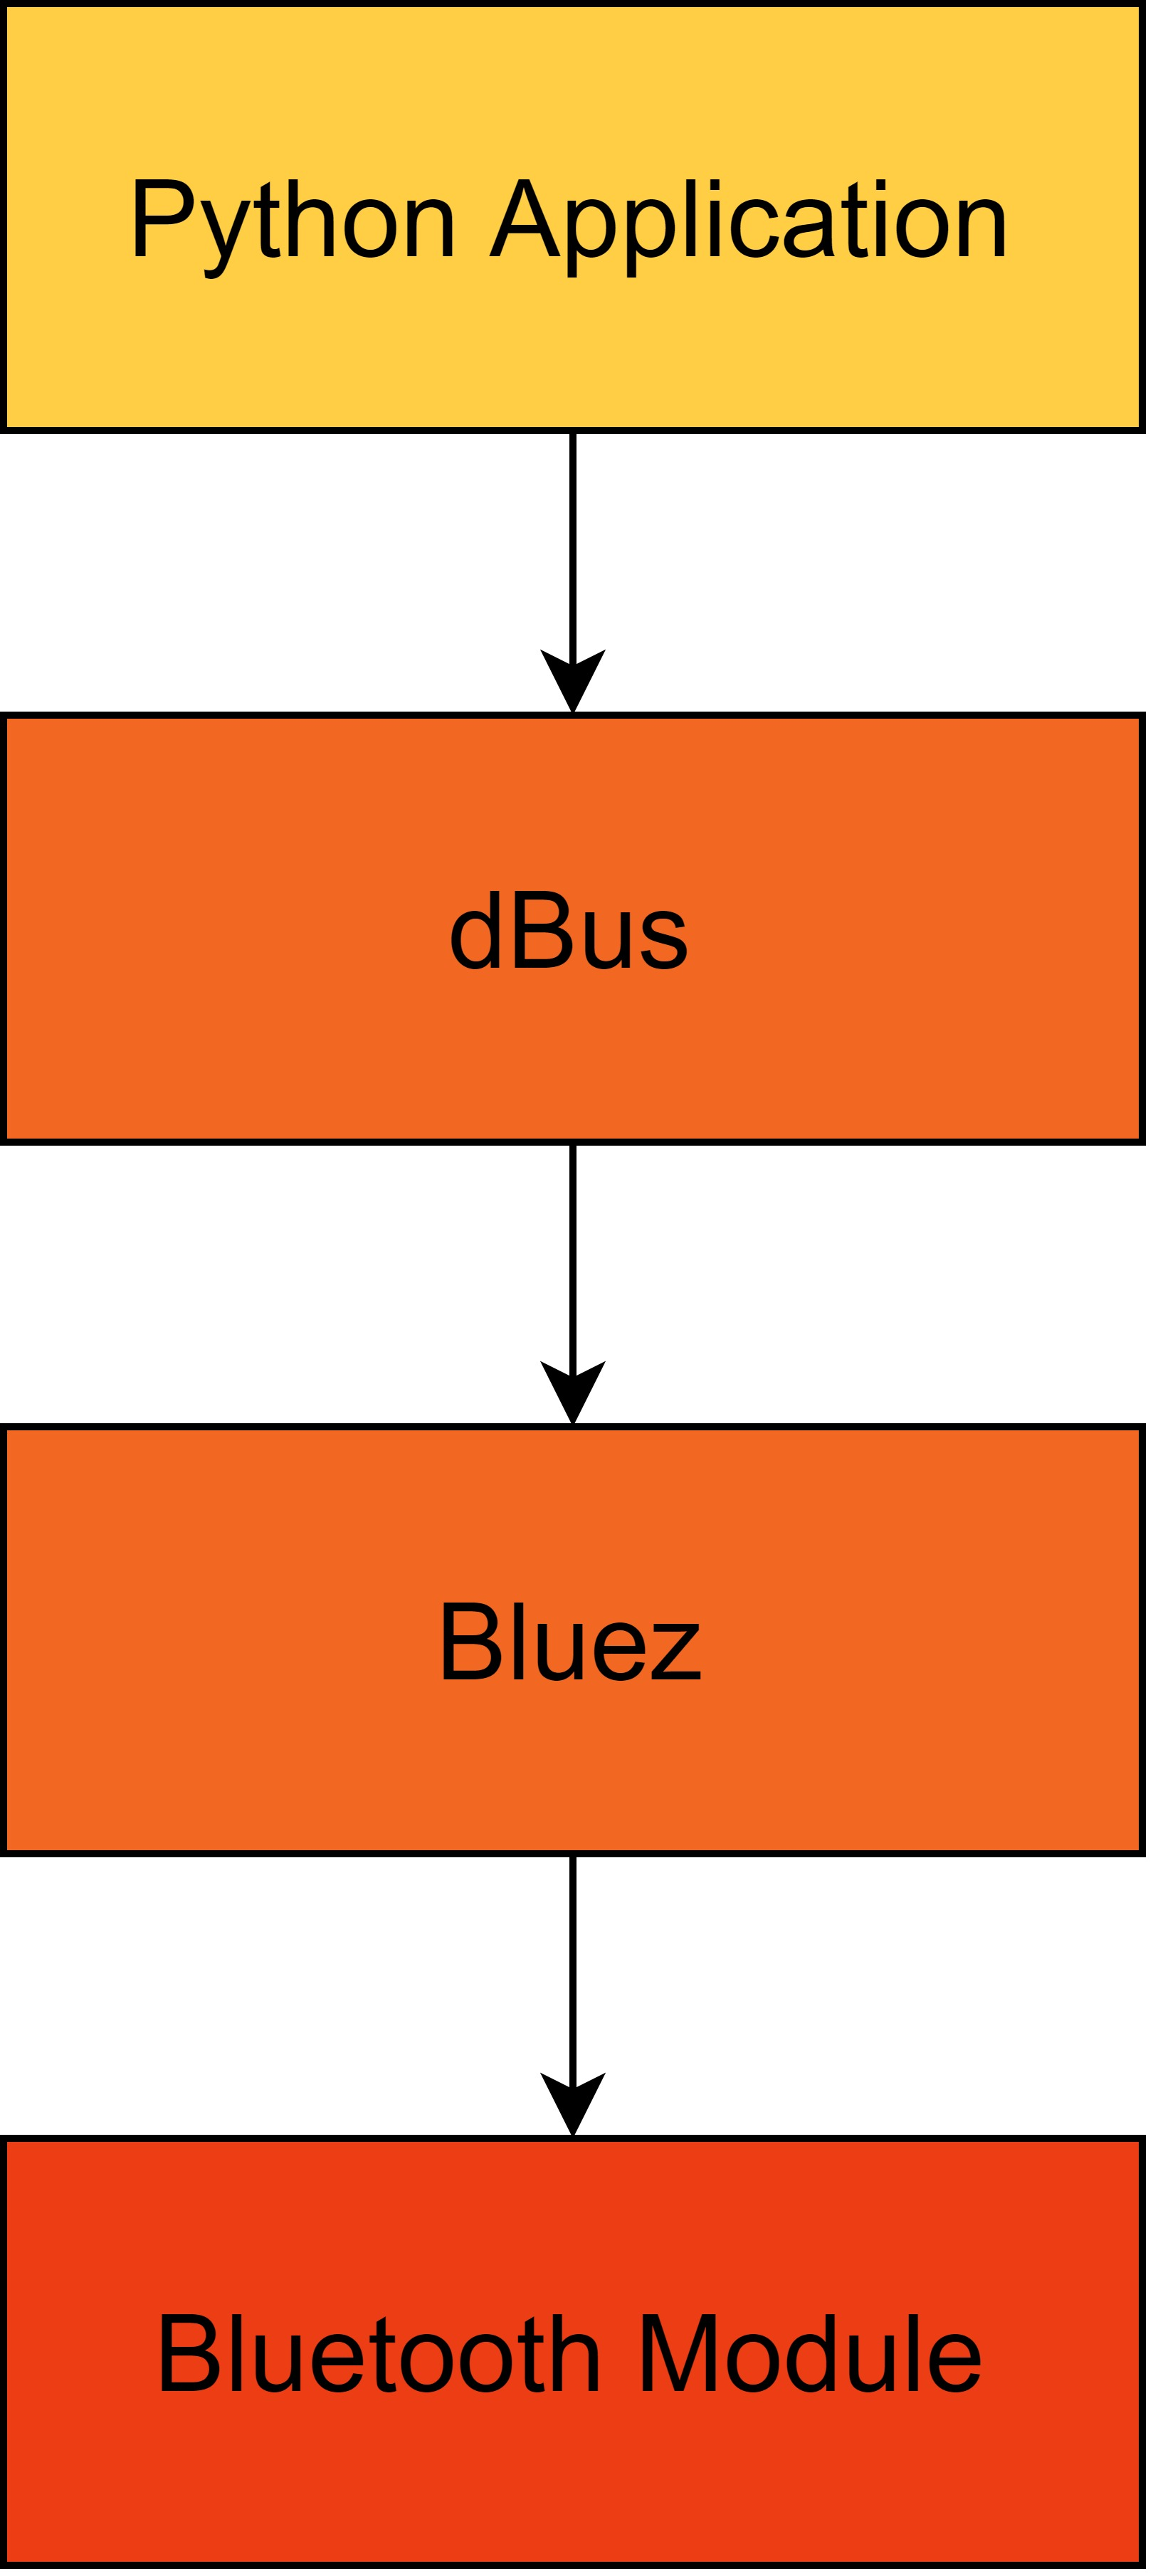
\includegraphics[height = \linewidth]{Abstraction.jpg}
		\caption{Abstraction Layers}
		\label{fig:abs}
	\end{subfigure}%
	\begin{subfigure}{.4\textwidth}
		\centering
		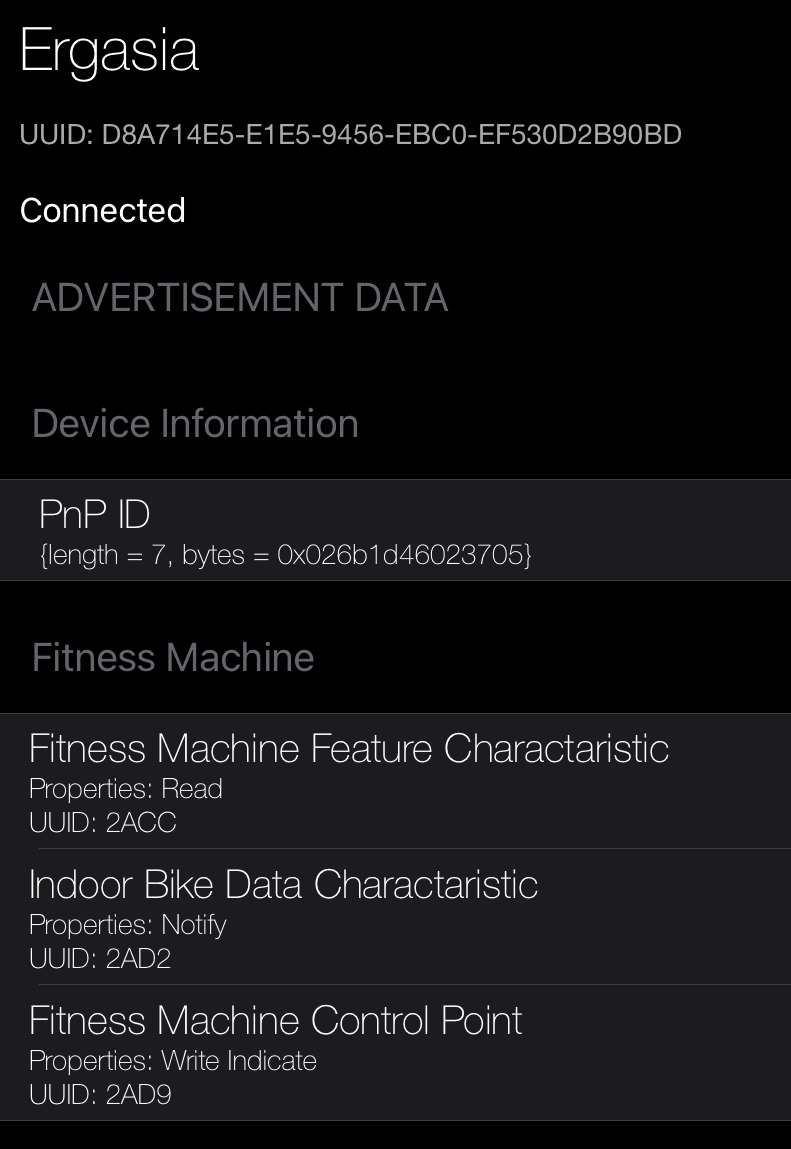
\includegraphics[height = \linewidth]{LightBlue.jpg}
		\caption{Light Blue Scan Results}
		\label{fig:blt}
	\end{subfigure}
	\caption{\ac{ble} Communication}
	\label{fig:bt}
\end{figure}

\vspace*{-0.9cm}

Figure~\ref{fig:abs} shows the levels of abstraction that were leveraged in the design of the communication protocol for the application. The application utilises the \ac{dbus} in order to make \acp{rpc} to Bluez. Bluez is the official Linux Bluetooth protocol stack and controls the Bluetooth operations of the system. \citep{Lee:2020}

\section{Application Outline}

Figure~\ref{fig:main} shows the flow diagram for the start of the application as soon as the Raspberry Pi is powered on. The application initializes all interrupts and callbacks then hands the operation back to the system process handler. This is indicated by the sleep block at the end of the diagram.

The application handles all different events with callbacks and interrupts. One such event is the transmission of speed and power data once every second. Figure~\ref{fig:spdsend} shows the logic flow for this callback when the set timer reaches one second. At the end of the callback, control is again handed back to the system process controller.

\begin{figure}[H]
	\centering
	\begin{subfigure}[t]{.4\textwidth}
		\centering
		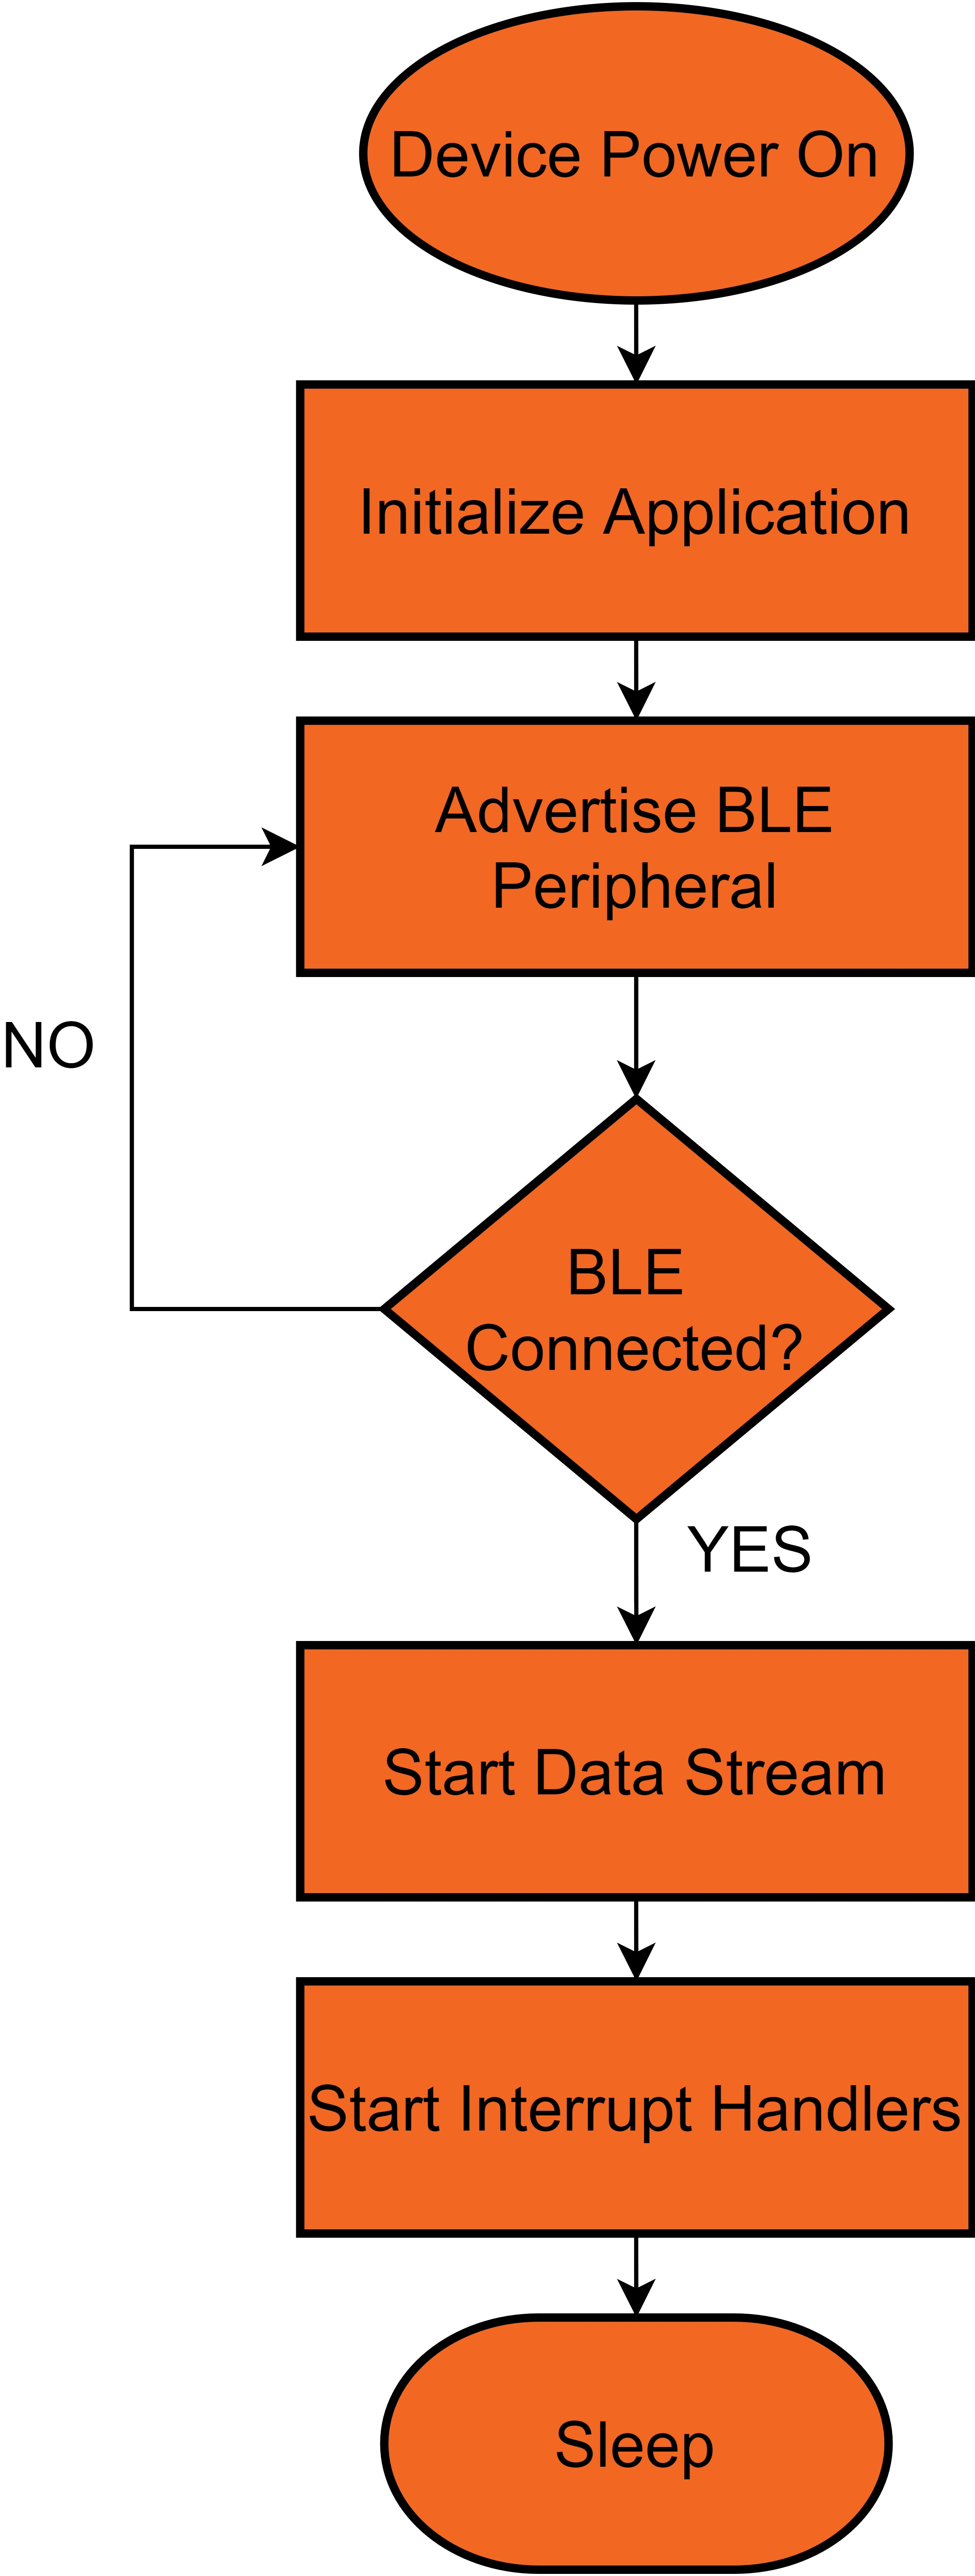
\includegraphics[height=1.5\textwidth]{MainLoop.jpg}
		\caption{Main Program}
		\label{fig:main}
	\end{subfigure}%
\hfill
	\begin{subfigure}[t]{0.5\textwidth}
		\centering
		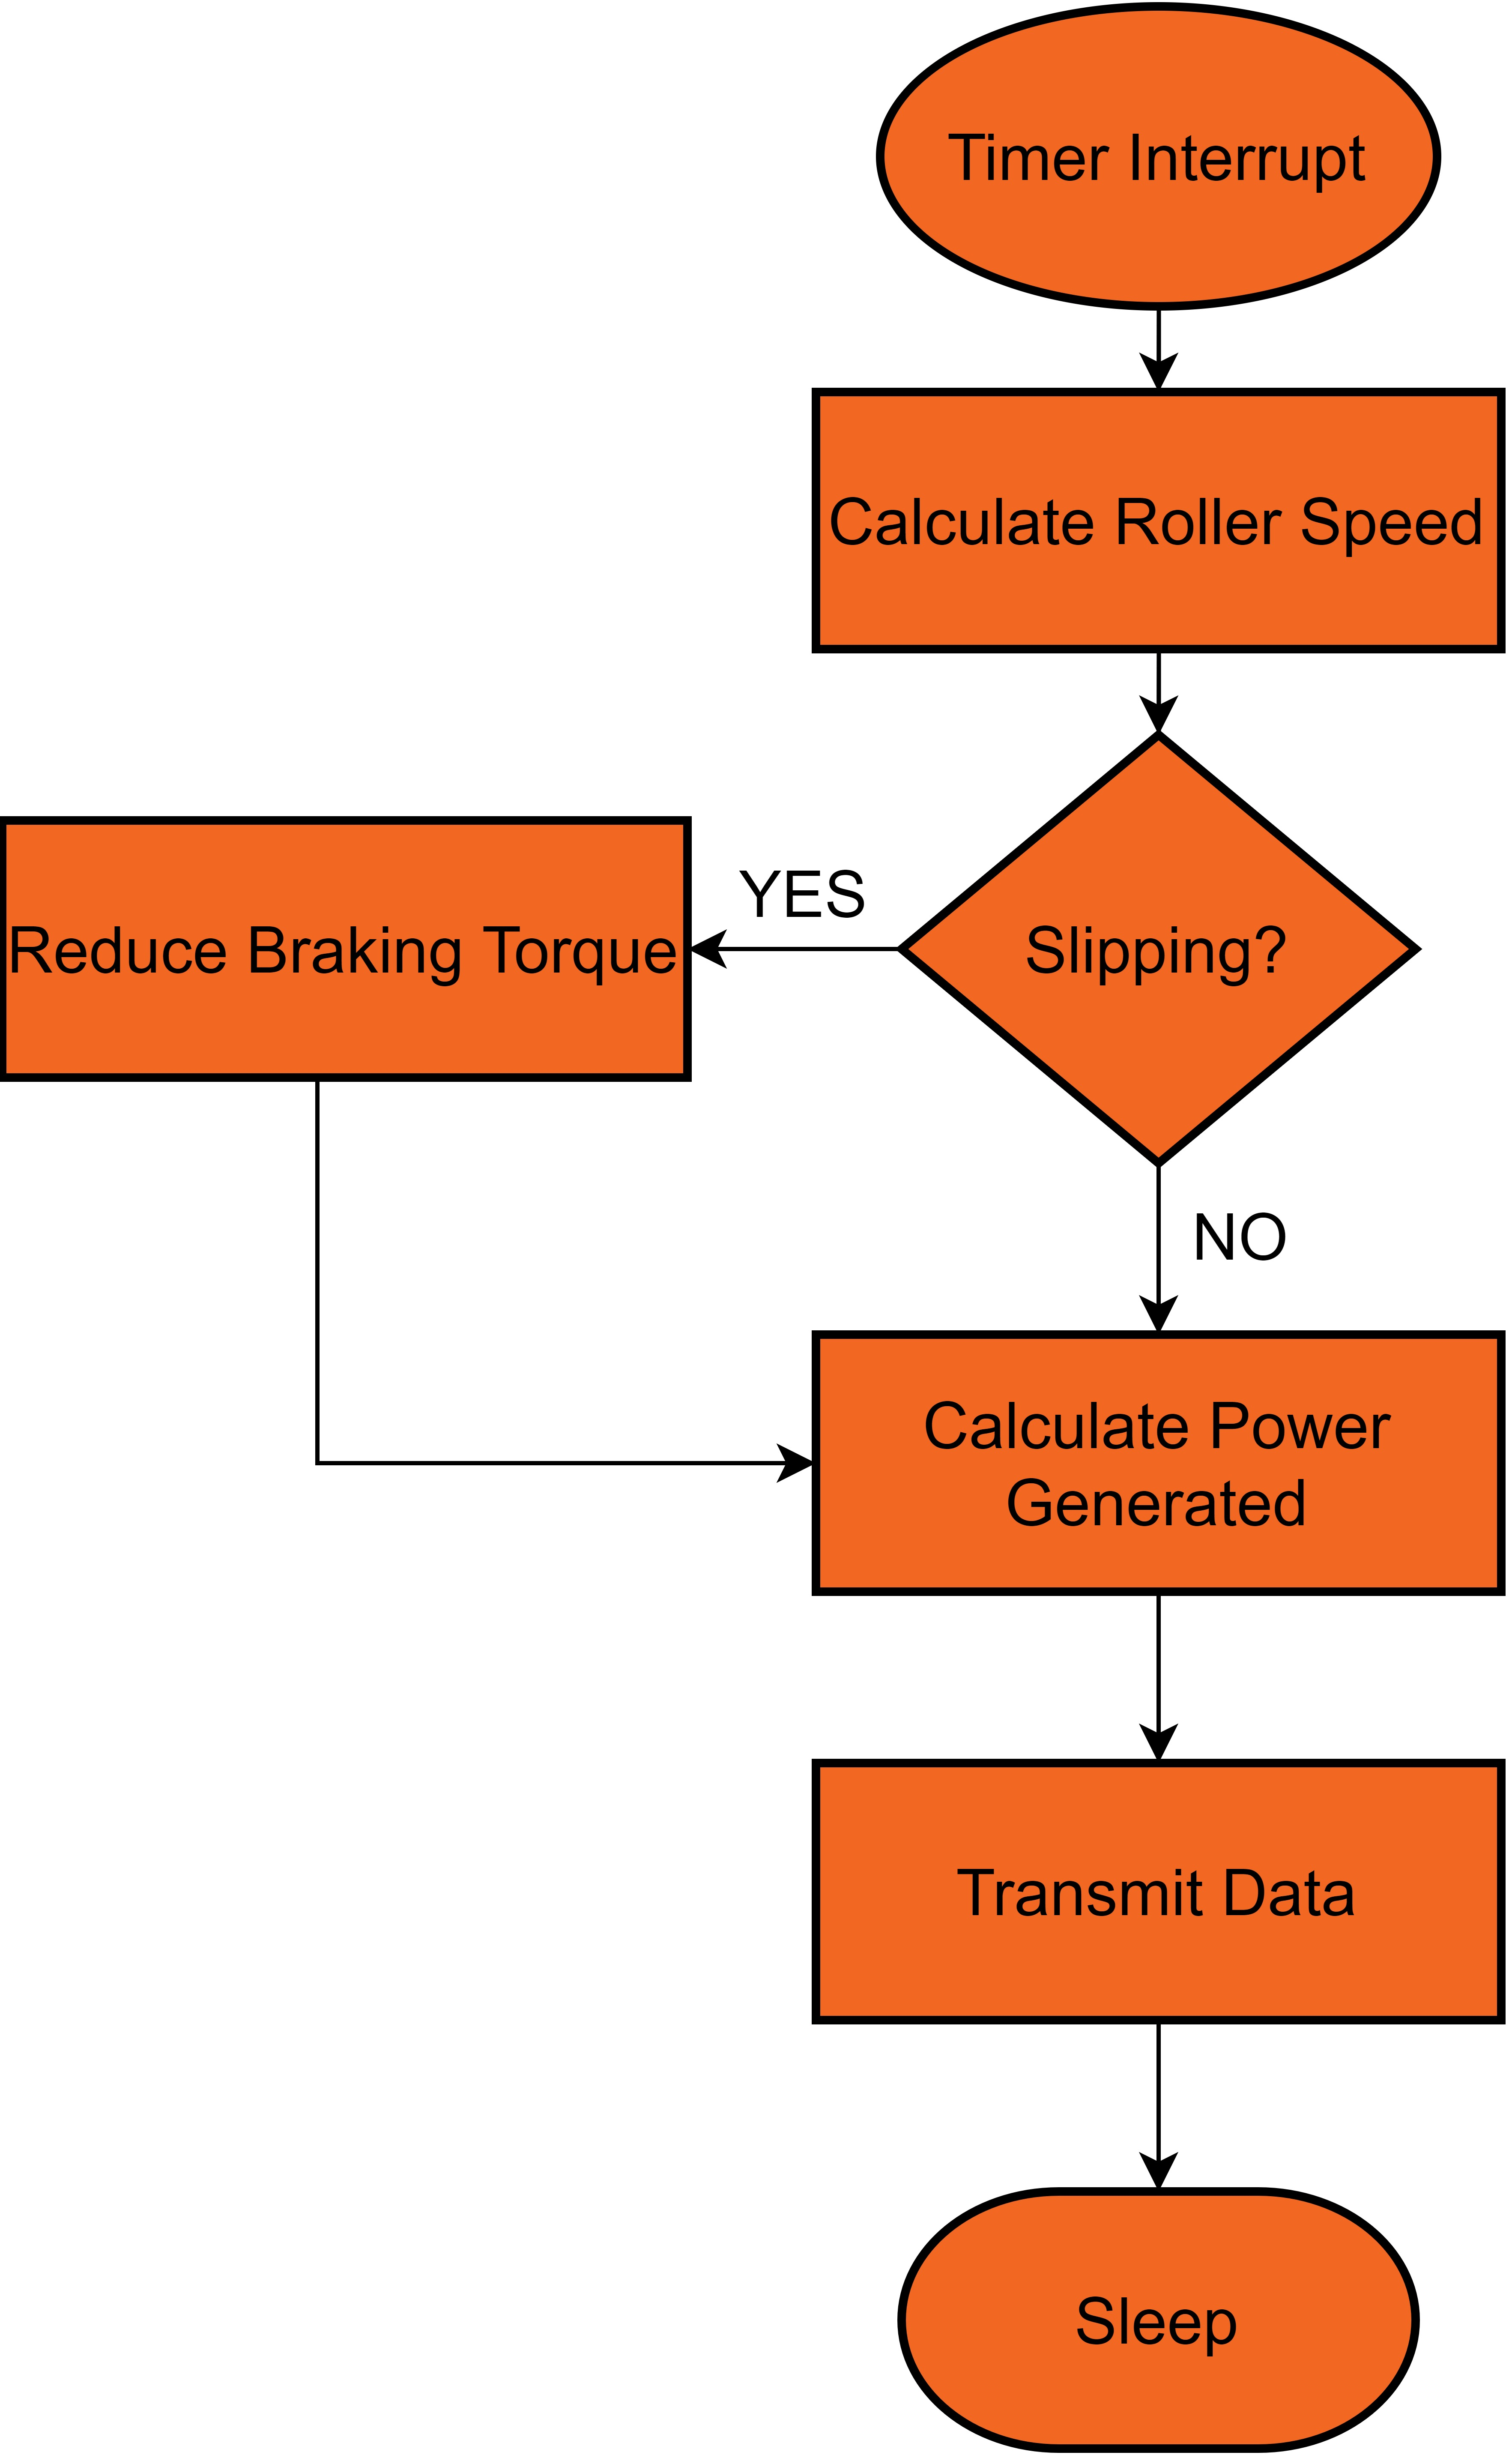
\includegraphics[height=1.1\textwidth]{DataStream.jpg}
		\caption{Data Stream}
		\label{fig:spdsend}
	\end{subfigure}
	\caption{Program Flow Diagrams}
	\label{fig:flow}
\end{figure}

%\section{Power Calculations}
%
%The power can be calculated if the braking torque applied to the power roller is known. Similarly, when \ac{sim} parameters are received from Zwift, the required braking torque to be applied by the brake needs to be calculated. The rolling resistance ($F_r$) can be determined using Equation~\ref{eq:Fr}, where the 
%
%\begin{equation}
%	f_r = W_{normal} * C_{rr}
%	\label{eq:Fr}
%\end{equation}
%
%\begin{equation}
%	W_{normal} = \tan(Grade) W
%	\label{eq:Wn}
%\end{equation}
%
%\begin{figure}[H]
%	\begin{center}
%		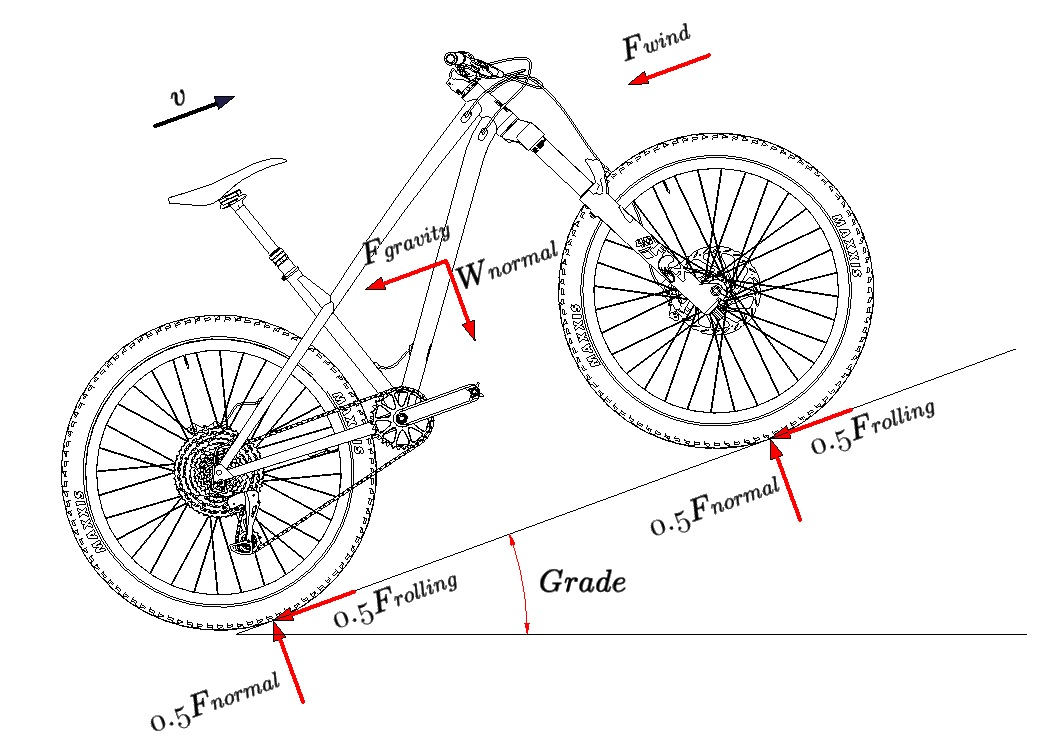
\includegraphics[width=0.4\textwidth]{SIM.jpg}
%		\caption{Cycling Physics Illustration}
%		\label{fig:sim}
%	\end{center}
%\end{figure}


